%%%%%%%%%%%%%%%%%% ATLAS

\section{The ATLAS Experiment}
\label{sed:cern:atlas}

ATLAS (A Toroidal LHC ApparatuS)\cite{atlas:atlas} is the largest of the LHC detectors: as it is shown in Fig. \ref{fig:atlas:atlas} it measures 44 meters in length and 25 meters in height, and its weights is about 700 tons. To be fully functional in the LHC environment,  ATLAS needs to be fast as it needs to be able to resolve the collisions resulting from consecutive bunches (which are interspaced by 25 ns) and radiation resistant. 

\begin{figure}[ht]
\centering
\subfigure{\includegraphics[width=0.85\textwidth]{figures/atlas/atlas}}
\caption{Computer-generated image of the ATLAS inner detector. Figure from Ref. \cite{atlas:atlas}}
\label{fig:atlas:atlas}
\end{figure}

The ATLAS physics program covers a large variety of topics: 
\begin{itemize}
\item Standard Model processes can be measured at the LHC at energies never reached before, and being sensitive to them is essential both to provide accurate measurements and to use them as candles to calibrate the detector. 
\item The discovery of the Higgs boson was one of the main goals of the LHC, and after its observation in 2013 the focus moved on measuring its properties. 
\item Top quarks are produced in large amount at the LHC, and the study of the properties of this particle can both probe the SM and set limits on BSM theories.
\item The LHC offers an incredible opportunity to discover BSM physics, and ATLAS needs to be ready to identify its signs.
\item Despite the ALICE detector is specifically designed to study heavy-ion collisions, ATLAS also carries out an heavy-ion program.
\end{itemize}

To cope with the wide range of types and energies (from few GeV to several TeV) of the particles that need to be identified, ATLAS relies on a sequence of subdetectors nested in a cylindrical geometry, that follow the general schema discussed in Section \ref{sec:detectors:identification}: close to the interaction point we find the inner detector (ID), embedded in a solenoidal magnetic field of 2 T. The following layers are the electromagnetic and the hadronic calorimeters (ECal and HCal), and the outermost part is occupied by the muon system, where muons are bent by a 4-T toroidal magnetic field. All of these components are described in the next sections.

\subsection{Coordinate System}

ATLAS uses a right-handed coordinate system, with its origin at the nominal interaction point. The $z$-axis follows the beam direction, while in the transverse plane the $y$-axis points upward and the $x$axis toward the LHC center. Positive and negative values of the $z$-axis identify respectively the A-side and the C-side of the detector. When spherical coordinates are used, the \textit{azimuthal angle} $\phi$ is defined starting from the $x$-axis, and ranges between $-\pi$ and $\pi$; the \textit{polar angle} $\theta$ is defined starting from the $z$-axis and takes values between $0$ and $\pi$. Often the polar angle is substituted by the \textit{pseudorapidity}: 
 
\begin{equation}
\label{eq:cern:eta}
\eta = - \ln \tan \frac{\theta}{2}
\end{equation}

which, in the limit of massless particles, is equivalent to the \textit{rapidity}:

\begin{equation}
\label{eq:cern:y}
y = \frac{1}{2} \ln \frac{E + p_z}{E - p_z} \; ,
\end{equation}

where $E$ is the energy of the particle and $p_z$ its momentum projected on the $z$-axis. The $\eta$-$\phi$ plane is used to define the angular separation of two objects in the detector:

\begin{equation}
\label{eq:cern:dR}
\Delta R = \sqrt{ \Delta \phi^2 + \Delta \eta^2  } \; .
\end{equation}

Since protons are composite particles, and the hard scattering happens between its constituents, the longitudinal momentum of the partons is unknown. It is therefore useful to define the \textit{transverse momentum} as the projection of the momentum on the ($x$,$y$) plane: 

\begin{equation}
\label{eq:cern:pt}
p_T = \sqrt{p_x^2 + p_y^2} \; ,
\end{equation}

where $p_{x(y)}$ are the projection of the momentum along the $x$-($y$-)axis.




\subsection{Magnet System}

The two segments of the ATLAS detector that are dedicated to tracking, the ID and the muon spectrometers, are embedded in two separate magnetic fields. A schematic overview of the ATLAS magnetic system is shown in Fig. \ref{fig:atlas:magnet}.
\label{sec:cern:atlasmagnets}
\begin{figure}[ht]
\centering
\subfigure{\includegraphics[width=0.35\textwidth]{figures/atlas/magnets}}
\caption{Layout of the ATLAS magnet system. Figure from Ref. \cite{Goodson}}
\label{fig:atlas:magnet}
\end{figure}

As discussed in Section \ref{sec:dec:tracking}, the magnetic field configurations that are more suitable for a detector with cylindrical symmetry are solenoidal and toroidal. The bending of the charged particles in the ATLAS ID is caused by an axial 2-T solenoidal field, provided by the \textit{central solenoid} \cite{YAMAMOTO200853}. This magnet is 5.8-m long, has an inner diameter of 2.46 m and an outer diameter of 2.56. The wounded coil is made of an Al-stabilised NbTi conductor, and is powered with a 7.73 kA current. 


In the muon system, a solenoid would be disadvantageous in the measurement of forward muons, since the resultant magnetic field would not be perpendicular to the trajectory of those particles. The usage of a toroid to provide the outer magnetic field solves this problem. The main drawback of this choice is that, in order to obtain the same intensity of the magnetic field, a toroid needs more current than a solenoid (20.5 kA for 4 T).
The ATLAS toroid system is divided into two subsystems, to allows for an easier design, as well as access to the core part of the detector.
The \textit{barrel toroid} \cite{ATLAS:1997ac} provides a peak field of 3.9 T in the cylindrical shell between the calorimeters and the end of the muon spectrometer, and consists of eight coils contained in individual vacuum vessels.  
The \textit{end-cap toroids} \cite{ATLAS:1997ab} provide the magnetic field necessary to bend the muons in the end-cap region of the spectrometer, and each of them consists of eight coils building a single cold mass, originating a peak field of 4.1 T. 



\subsection{Inner Detector}

The main purposes of ATLAS inner detector \cite{ATLAS:1997ag,ATLAS:1997af} are to provide a good momentum resolution of the charged particles produces in the collisions and to allow the determination of secondary vertexes. The size of the ID is determined on one side by the beam pipe and on the other side by the beginning of the ECal. The total length is 5.4 m, that allows a coverage up to $|\eta|<$2.5.
The ID is divided into a barrel ID, whose schema is shown in Fig. \ref{fig:atlas:id}, and two end-cap regions, covering respectively the pseudorapidity regions $|\eta|<$1.2 and 1.2$<|\eta|<$2.5. In both, a mixture of gaseous and silicon detectors is used to maximize the performance and reduce the costs. The three components that compose the ID are the pixel detector, the semi-conductor tracker and the transition radiation tracker, discussed in the following paragraphs.

\begin{figure}[ht]
\centering
\subfigure{\includegraphics[width=0.65\textwidth]{figures/atlas/inner_detector}}
\caption{Layout of the ATLAS inner detector. Figure from Ref. \cite{Potamianos:2016ptf}}
\label{fig:atlas:id}
\end{figure}


\subsubsection*{Pixel Detector}
The innermost layer of the ID is the \textit{pixel detector}, divided into barrel and end-cap regions. During the Long Shutdown after the LHC Run1, the ID was subject to important upgrades \cite{Potamianos:2016ptf}. The main one is the addition of a fourth pixel layer in the barrel, in addition to the three already existing ones, the insertable B-Layer (IBL) \cite{Capeans:1291633}, that is positioned 3.33 cm away from the interaction point. In order to locate a detector so close to the interaction point, the beam pipe had to be replaces with a thinner one. The IBL is 72.4 cm long along the $z$ direction, and consists of 14 staves that provide full coverage in azimuthal angle. Each stave contains 20 modules, 12 with planar silicon sensors and 8 with 3D pixel sensors \cite{1748-0221-7-11-P11010}, and each module has 144$\times$328 pixels with the size of 50$\times$250 $\mu$m$^2$, for a total of over 12 million pixel in the entire IBL. The size of the pixels leads to a resolution of 40 $\mu$m in the longitudinal direction and 8 $\mu$m in the perpendicular one. The three outer pixel layers are located at 5.05, 8.85 and 12.5 cm from the interaction point. Each module contains 80 pixels of 50$\times$400 $\mu$m$^2$, leading to a spatial resolution of 115 and 10 $\mu$m respectively in the longitudinal and transverse direction. 
The two end caps, on the two sides of the detector, consist of three wheels each, with a radius of 34 cm and located at 49.5, 58.8 and 65.0 cm from the interaction point. 
To ensure a good performance, the ID detectors need to be kept at a low and stable temperature, between -15$^{\circ}$ C and 5$^{\circ}$ C for the IBL, between -15$^{\circ}$ C and -10$^{\circ}$ C for the other layers.

\subsubsection*{Semi-Conductor Tracker}
The ATLAS Semiconductor Tracker (SCT) is composed by 4088 silicon micro-strip modules with binary readout mounted on carbon fibre composite structures and is organized in four cylinders in the barrel and nine disks in each of the forward regions \cite{Jackson:sct}. The cylinders have a radii of 30.0, 37.3, 44.7 and 52.0 cm and provide a coverage for $|\eta|<$1.1-1.4, while the disks cover the region with 1.1-1.4$<|\eta|<$2.5. 
2112 of the 4088 SCT modules are in the barrel, and contain single-sided p-in-n silicon strips, with a pitch of 80 $\mu$m. In the module, the strip sensors are positioned back to back with an angle of 40 mrad, to be able to access information on the $z$-coordinate as well. The end-cap modules use strips with width between 56.9 and 94.2 $\mu$m. These choices lead to a spatial resolution of 17 $\mu$m in the transverse direction and 580 $\mu$m in the longitudinal one. Also the SCR components need to be kept at a low temperature, between -15$^{\circ}$ C and -5$^{\circ}$ C.

\subsubsection*{Transition Radiation Tracker}

The transition-radiation tracker (TRT) is the outermost layer of the ID. In the barrel it consists of 52544 straw tubes with a length of 1.5 m disposed parallel to the beam direction, while each end-cap contains 122880 straw tubes 0.4-m long disposed perpendicularly to the beam axis. Each tube is 4 mm in diameter, and has in the inside gold plated tungsten wire as anode with a diameter of 31 $\mu$m. The tubes are filled with a mixture of 70\% Xe, 27\% CO$_2$ and 3\% O$_2$; due to a gas leakage, in 2016 part of the TRT tubes have been filled with a cheaper mixture of 80\% Ar and 20\% CO$_2$. The TRT is the only subdetector of the ID that has a pseudorapidity coverage up to $|\eta|<$2. The TRT provides tracking information only in the (r-$\phi$) plane, with a resolution of 130 $\mu$m.


\subsection{Calorimeters}

The ATLAS calorimeter system is located outside the ID and the magnetic field of the solenoid, as shown in Fig. \ref{fig:atlas:calo}. The electromagnetic calorimeter (ECal) is closer to the interaction point, while the hadronic calorimeter (HCal) is on the outside; both systems have a barrel and an end-cap part. 
The combined thickness of the calorimeter system is about 11 interaction lengths to allow a good reconstruction of the energy imbalance in the event, which is a measure of the energy carried away by neutral weakly-interacting particles, and the total pseudorapidity coverage is up to $|\eta|<4.9$. 

\begin{figure}[ht]
\centering
\subfigure{\includegraphics[width=0.75\textwidth]{figures/atlas/calorimeters}}
\caption{Layout of the ATLAS calorimeter system. Figure from Ref. \cite{atlas:atlas}}
\label{fig:atlas:calo}
\end{figure}

Table \ref{tab:atlas:cal:reso} shows the energy resolution of the different subsystems. As expected from the discussion in Section \ref{sec:dec:calo}, the resolution is better for electromagnetic showers than for the hadronic ones. For example, a 1-GeV particle detected in the ECal has an energy resolution of about 19\%, while 50\% (100\%) if detected in the HCal barrel (end-caps). On the other hand, a 1-TeV particle has an energy resolution of 0.7\% in the ECal and 3\% (10\%) in  HCal barrel (end-caps), and in this case the resolution is dominated by the constant term.

\begin{table}[ht]
\begin{center}
\begin{tabular}{c c }
\hline
Component & $\sigma_E / E$ \\
\hline 
\hline
ECal & 0.1$/\sqrt{E[GeV]}$ + 0.17$/E$ 0.007 \\ % chiara: cite LAr TDR
\hline
HCal barrel & 0.5$/\sqrt{E[GeV]}$ + 0.03 \\
\hline
HCal end caps & 1$/\sqrt{E[GeV]}$ + 0.1 \\
\hline
\end{tabular}
\end{center}
\caption{Energy resolution of the ATLAS calorimeter systems.}
\label{tab:atlas:cal:reso}
\end{table}

\begin{figure}[ht]
\centering
\subfigure[]{\includegraphics[width=0.495\textwidth]{figures/atlas/barrel_em.pdf}}
\subfigure[]{\includegraphics[width=0.495\textwidth]{figures/atlas/fisarmonica.jpeg}}
\caption{(a) Schema of a barrel module of the ATLAS ECal. (b) Accordion shape of the metal plates of the ECal.}
\label{fig:atlas:lar}
\end{figure}

\subsubsection*{Electromagnetic Calorimeter}

The ECal is a sampling calorimeter with liquid argon (LAr) as active material and lead plates as absorber, both in the barrel and in the end caps. The lead plates have a characteristic accordion shape and, in the barrel, are oriented in the radial direction. Before the ECal, a presampler provides the information necessary to reconstruct the amount of energy lost in the passive material of the solenoid. The design of a LAr barrel module is shown in Fig. \ref{fig:atlas:lar}(a), where it is possible to see the segmentation in three layers with decreasing granularity: the first layer is finely segmented in pseudorapiditu, with strips of $\Delta\eta \times \Delta\phi = $ 0.0031 $\times$ 0.098. The second layer has towers of $\Delta\eta \times \Delta\phi = $ 0.025 $\times$ 0.025 to measure the clusters, while the third layer has broader towers of $\Delta\eta \times \Delta\phi = $ 0.05 $\times$ 0.0245 to provide an estimate of the energy propagating beyond the ECal. In the LAr barrel offers pseudorapidity coverage up to $|\eta|<$1.475, and the thickness of the detector varies from 22 $X_0$ at $\eta=0$ to 33 $X_0$ at $|\eta|=1.3$. 
Each of the two end-cap regions consists of two coaxial wheels, of eight module each, that cover the region 1.375$<|\eta|<$3.2, with a thickness varying between 26 and 36 $X_0$ for the inner wheel, 24 and 38 $X_0$ for the outer wheel. The end-cap modules are divided into two layers, again with decreasing granularity.


\subsubsection*{Hadronic Calorimeter}

The hadronic calorimeter is composed of three subsystems with different technologies: the tile barrel calorimeter (TileCal) is a sampling calorimeter with plastic scintillator as active material and steal as absorber, the hadronic end-cap calorimeter (HEC) uses copper as absorber and liquid argon as scintillator, while the forward calorimeter (FCal) uses again liquid argon in the active layer but has tungsten rods embedded in a copper matrix as absorber. The choice of the materials is driven by having detectors more resistant to radiation in the forward region, where the flux of particles is more abundant. 

TileCal covers the pseudorapidity region with $|\eta|<$1.7, and is divided into a central long barrel (LB), 5.8-m long, and two extended barrels (EB), 2.6-m long; the TileCal inner radius is 2.28 m, and the outer radius 4.25 m. Each barrel is divided in 64 modules, disposed on the $\phi$ direction and each having the size of 0.1 radians. Each module is further segmented radially into three layers with thicknesses of about 1.5, 4.1 and 1.8 interaction lengths in the LB and 1.5, 2.6 and 3.3 interaction lengths in the EB; a schematic of one module is shown in Fig. \ref{fig:atlas:tile}(a). Ionizing particles passing through the plastic scintillator (polystyrene) produce ultra-violet light, which is then collected at the two edges of each tile and converted to the longer wavelength of visible light by wavelength-shifting fibers. The fibers, with a diameter of 1 mm each, transmit the light to the readout photomultiplier tubes (PMTs) located in the grinder.

\begin{figure}[ht]
\centering
\subfigure[]{\includegraphics[width=0.495\textwidth]{figures/atlas/tile.pdf}}
\subfigure[]{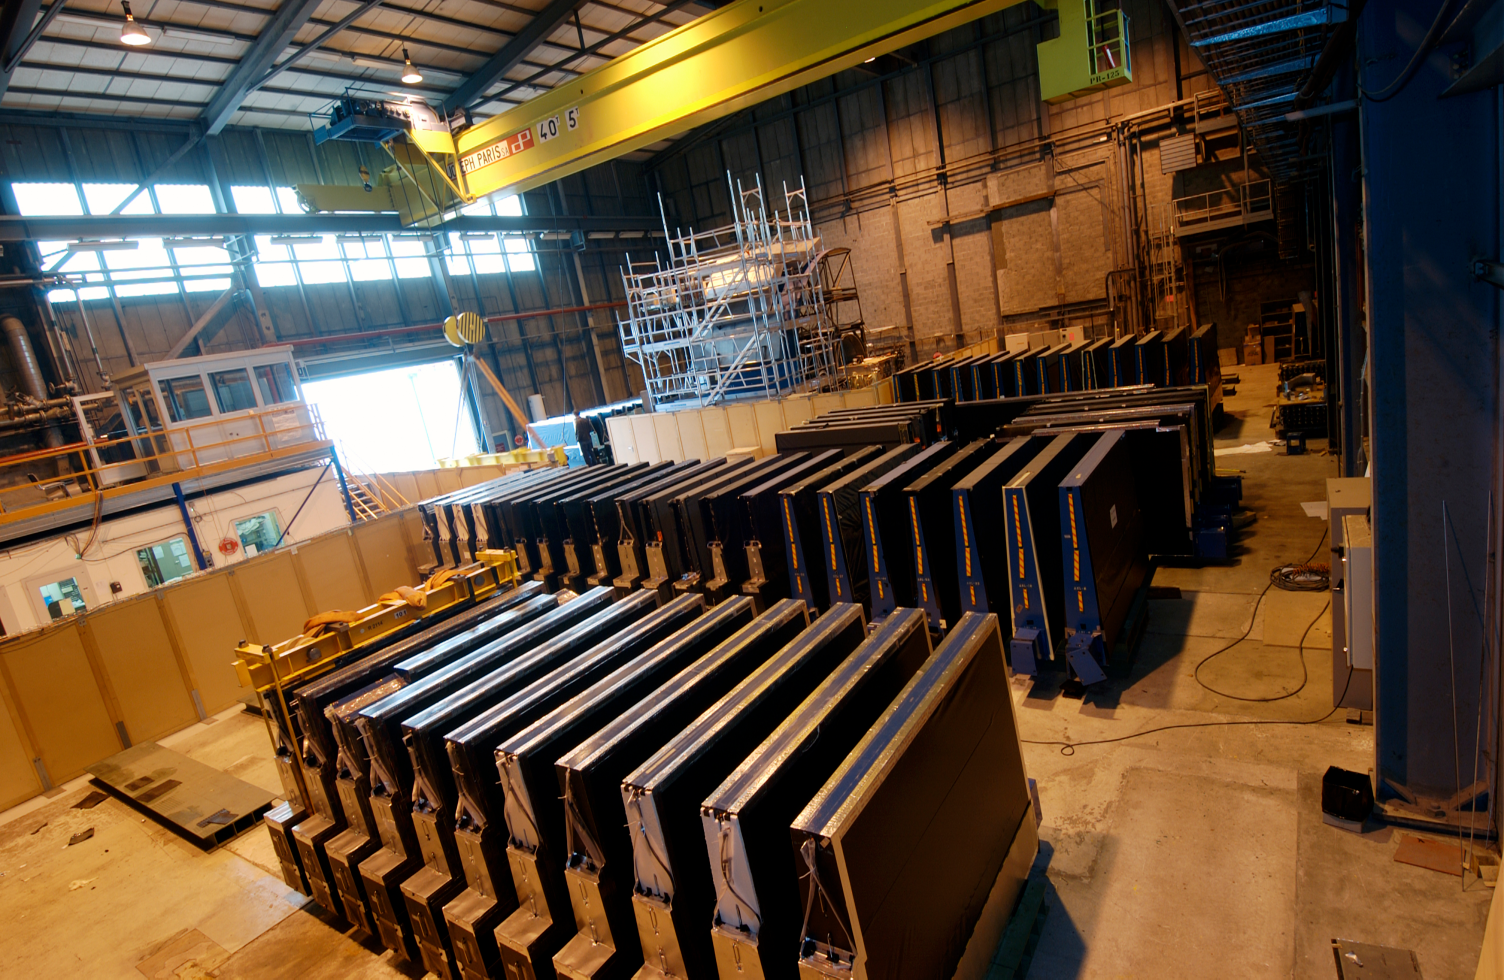
\includegraphics[width=0.495\textwidth]{figures/atlas/tile_pic.pdf}}
\caption{(a) Schematic representation of a TileCal module and its interface with the optical readout. (b)}
\label{fig:atlas:tile}
\end{figure}

An approximately projective geometry, shown in Fig. \ref{fig:atlas:tile_cells}, is provided by the grouping of the readout fibres into the PMTs: this defines a cell structure, and each cell has dimension $\Delta\eta \times \Delta\phi = $ 0.1 $\times$ 0.1 in the first two layers and $\Delta\eta \times \Delta\phi = $ 0.2 $\times$ 0.1 in the third layer. Special cells cover the gap region between the LB and the EB: the gap scintillators in the pseudorapidity region 1.0$<|\eta|<$1.2 and crack scintillators in the region 1.2$<|\eta|<$1.6, in front of the LAr end caps.

\begin{figure}[ht]
\centering
\subfigure{\includegraphics[width=0.7\textwidth]{figures/atlas/tile_cells.pdf}}
\caption{Layout of the projective geometry of the TileCal cells.}
\label{fig:atlas:tile_cells}
\end{figure}

The HEC shares the same cryogenic system as the ECal end caps, and covers the region with 1.5$<|\eta|<$3.2. Liquid argon is more resistant to radiation than the plastic scintillator used in TileCal, and is therefore the preferred choice in the end-cap region. Each side of the HEC consists of two wheels with outer radius of 2.03 m, and each wheel is composed by 32 identical modules. The electromagnetic signal produced in the LAr is collected by catodes on the plates. 

The FCal provides coverage in the forward region with 3.1$<|\eta|<$4.9. The FCal modules are located at high pseudorapidity, at a distance of 4.7 m along the $z$-axis from the interaction point.


\subsection{Muon Spectrometer}

\begin{figure}[ht]
\centering
\subfigure{\includegraphics[width=0.65\textwidth]{figures/atlas/muon}}
\caption{Layout of the ATLAS muon system. Figure from Ref. \cite{atlas:atlas}}
\label{fig:atlas:muon}
\end{figure}

\subsection{Luminosity Detectors}

\subsection{Luminosity Determination and Uncertainty}

\subsection{Trigger System}
\label{sec:cern:trigger}

\subsection{ATLAS Performance Summary}

